\chapter{Framework user manual}
\label{app:framework_user_manual}

\section{Installing}
Before starting the installation, ensure that Python 3.7 or later is available on your machine. 
The framework uses the \texttt{poetry} Python package for dependency management, and it is necessary to first install this package via \texttt{python3 install poetry}. 
Then, the framework's dependencies can be installed by running the following command in the \texttt{framework} folder:
\begin{verbatim}
poetry install
\end{verbatim}

\section{Documentation}
The documentation of the neural framework \texttt{nf} package is provided in HTML format at \texttt{framework/docs/nf/index.html} and the same information is also available in PDF format at \texttt{framework/docs.pdf}.
Notice that this documentation is only of the framework itself and not the demonstrational scripts provided alongside it.
Please refer to the documentation itself for information on how to develop custom agents, problems, and experiments. 
Furthermore, the demonstrations explained in \ref{sec:neural_surfer_demos} provide starting points for how you could set up your own experiments.

If you wish to generate the documentation yourself, run
\begin{verbatim}
./generate_docs_html.sh
\end{verbatim}
from within the \texttt{framework} folder to generate the HTML documentation, or
\begin{verbatim}
./generate_docs_pdf.sh
\end{verbatim}
to obtain the PDF documentation. 
Note that the latter requires additional dependencies, namely \texttt{pandoc} and \texttt{xelatex}.

\section{Running the demonstrations}
\label{sec:neural_surfer_demos}
The neural framework package comes with three experiments for demonstration.
Each experiment runs all of the implemented agents on a different problem.
Notice, however, that the hyperparameters are varied depending on the problem to ensure that the agents are effective.
This was especially important for the simulated annealing agent.
Various metrics are visualised including weight and output spaces as well as training loss.
The following demonstrations are implemented:
\begin{itemize}
    \item \texttt{demo\_stripe\_problem.py} of the RBF stripe problem as given in \ref{sec:stripe_problem};
    \item \texttt{demo\_shallow\_problem.py} of a neural problem with a shallow excitation gradient (this problem was not analysed in this report but described in detail in Figure 7 and accompanying text of \texttt{research/progress/main.pdf}); and
    \item \texttt{demo\_simple\_problem.py} of a simple neural problem without local minima.
\end{itemize}

To run any of the implementations, simply execute the command
\begin{verbatim}
python3 demo_stripe_problem.py
\end{verbatim}
replacing \texttt{demo\_stripe\_problem.py} with one of the scripts listed above.
This will start a web server on port 5000 by default and open a web browser to \texttt{http://localhost:5000/} where the front end will be running.
The folder \texttt{framework/screenshots} contains a screenshot of each of the demonstrations.

There are a variety of command line options which are identical for these demonstrational scripts.
To obtain this information, simply run the script with the \texttt{-h} option appended.
Below is an example for the \texttt{demo\_stripe\_problem.py} script.
\begin{verbatim}
$ python3 demo_stripe_problem.py -h
usage: demo_stripe_problem.py [-h] [--batch-size EPOCH_BATCH_SIZE]
                              [--batches EPOCH_BATCHES] [--columns COLS]
                              [--port PORT]

A demonstrational tool for the neural framework

optional arguments:
  -h, --help            show this help message and exit
  --batch-size EPOCH_BATCH_SIZE
                        Number of epochs to train for per agent per batch
  --batches EPOCH_BATCHES
                        Number of batches of training to perform for each
                        agent
  --columns COLS        The number of columns that the visualisations should
                        be arranged
  --port PORT           The port to run the server on
\end{verbatim}

\section{Using the front end}
\label{sec:using_front_end}
As previously mentioned, when starting an experiment, a browser window will open with the front end.
The web page will contain a grid of visualisations. 
These visualisations will usually be line plots where the $x$ and $y$ axes can be arbitrary metrics.
The exact visualisations to be displayed are defined in the setup of the experiment (in an argument to the \texttt{run\_server()} method).

Initially, the plots will be empty when the page is loaded. 
This is because the agents will start training and the plot is only updated after a specific number of epochs, defined by the \texttt{batch\_size} command line argument.
These updates happen in real time as training progresses.
If the plot is updating too slowly, it is recommended to simply lower the value of \texttt{batch\_size}.

Each visualisation will include the metrics gathered on all agents, each of a different colour (but the colours are consistent for each plot).
You may each agent's visibility using the buttons at the top, as shown in \ref{fig:framework_front_end_screenshot}.
\begin{figure}
    \centering
    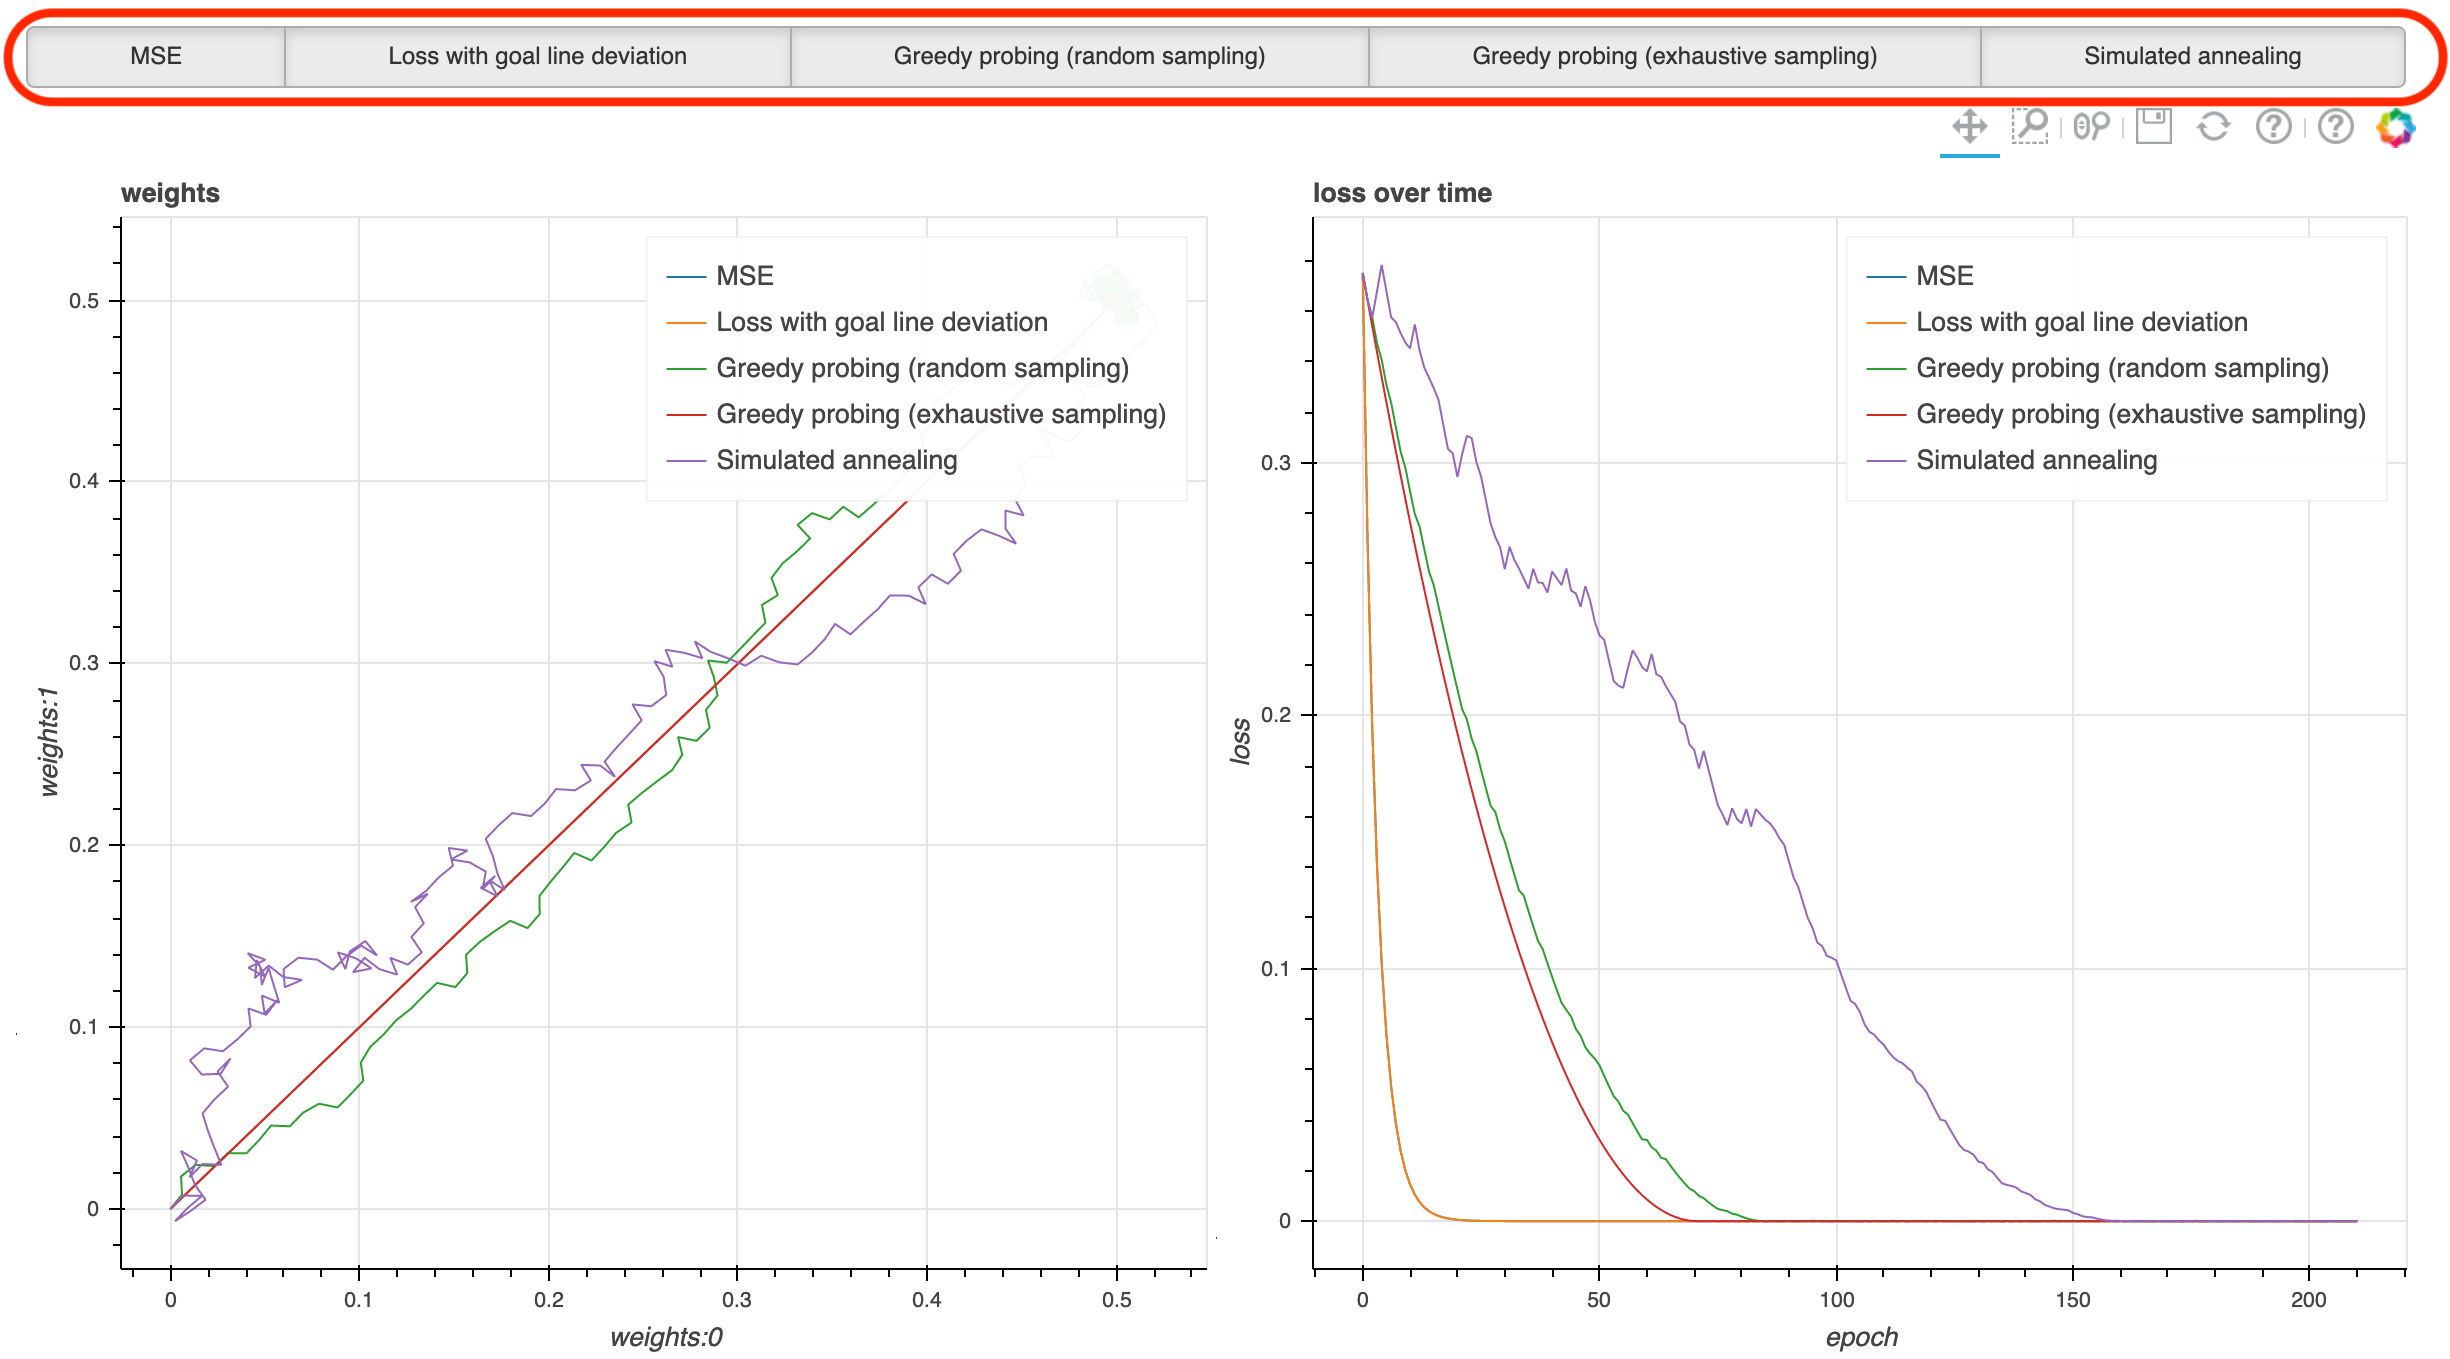
\includegraphics[width=\textwidth]{neural_framework_simple_problem_screenshot.png}
    \caption{Screenshot of the top part of the web page that constitutes the front end of the neural framework for the \texttt{demo\_simple\_problem.py} experiment. The area to the top marked in red contains the buttons for toggling each of the agents.}
    \label{fig:framework_front_end_screenshot}
\end{figure}
This will hide or show all plot lines with that agent's data.